\chapter{Main Part}
Lorem ipsum dolor sit amet, consetetur sadipscing elitr, sed diam nonumy
eirmod...

A list
\begin{enumerate}
 \item understand
 \item practise
 \item being capable of
\end{enumerate}


\section{Subchapter: second level}

Style sheet for continuous text. The figure~\ref{fig:ex} on page \pageref{fig:ex}
illustrates three drain curves of a two-phase defibrillator.

\begin{figure}[htb]
  \centering
  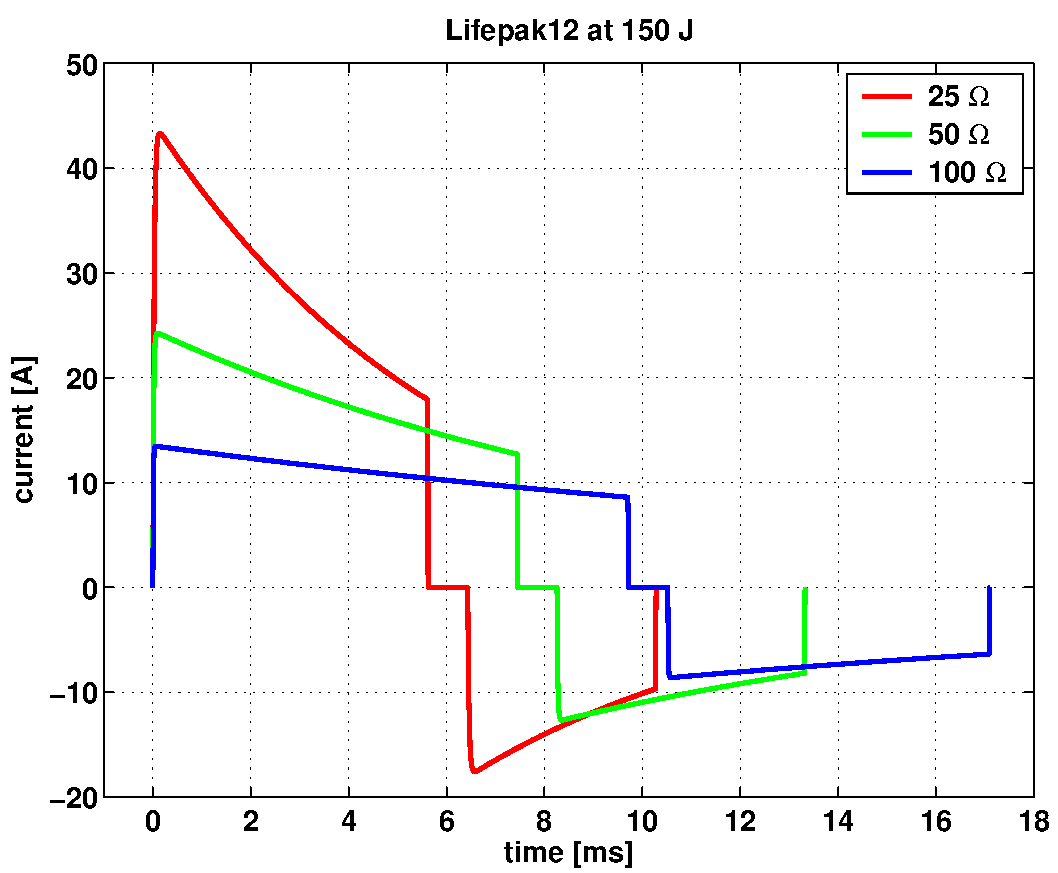
\includegraphics[width=6cm]{content/image/defi}
  \caption[Drain curve of a two-phase defibrillator]{Three drain curves. \\Source: own elaboration}
 \label{fig:ex}
\end{figure}


\section{Subchapter: second level}
Style sheet for continuous text. .
Now a footnote\footnote{This is a footnote.}
How many roots does the quadratic equation (\ref{equ:foo}) has?
\begin{equation}
 \label{equ:foo}
 x^2-2x+5=0.
\end{equation}
Two of Einsteins' most famous equations:
\begin{eqnarray*}
  E &= mc^2                                  \\
  m &= \frac{m_0}{\sqrt{1-\frac{v^2}{c^2}}}
\end{eqnarray*}


\subsection{Subsection third level}
Style sheet for continuous text. A simple table \ref{tab:sp} follows

\begin{table}[htb]
  \centering
  \begin{tabular}{ | l | l |c|}
    \hline
    Date      & Topic           & Room \\
    \hline\hline
    Monday     & Graph theory  & U1   \\
    \hline
    Thursday & Algebra         & MZB23\\
    \hline
  \end{tabular}
  \caption[Timetable]{Timetable of 2030.\\ Source: own elaboration}
  \label{tab:sp}
\end{table}

\subsubsection{Subsection: fourth level}
Style sheet for continuous text.

\paragraph{Subsection: fifth level}\mbox{}\newline
Style sheet for continuous text.

\paragraph{Subsection: fifth level}\mbox{}\newline
Style sheet for continuous text.


\section{Subchapter: second level}
Style sheet for continuous text. .
A recommended book \citep[vgl.][Chapter 2]{Chvatal1983} and an interesting article \citep{Einstein1905} of a famous man.


\chapter{[Another Chapter of the Main Part]}

\section{Subchapter: second level}
Style sheet for continuous text.

\subsection{Subchapter: third level}
Style sheet for continuous text.

\subsubsection{Subchapter: fourth level}
Style sheet for continuous text.

\paragraph{Subchapter: fifth level}\mbox{}\newline
Style sheet for continuous text.

\paragraph{Subchapter: fifth level}\mbox{}\newline
Style sheet for continuous text.


\chapter{[Last chapter]}
Style sheet for continuous text.
